\section{Оптический магнетизм}

Оптическим магнетизмом называют возбуждение в материалах ненулевого магнитного дипольного момента взаимодействующим электромагнитным излучением на оптических частотах.

Материалам, встречающимся в природе, часто присуща диэлектрическая проницаемость, значительно отличающаяся от вакуумной в оптическом диапазоне. Но при этом их магнитная проницаемость на тех же длинах волн как правило близка к своему значению в свободном пространстве \cite{Shalaev2007}. Подобное поведение связано с тем, что степень взаимодействия атома с магнитной компонентой поля пропорциональна магнетону Бора $\mu_B = e \hbar/2 mc = \alpha e a_0 /2$, где $\alpha \cong 1/137$~--- постоянная тонкой структуры. Из этого вытекает что отклик атома на магнитное поле слабее, нежели отклик на электрическую компоненту.

Выходом может стать создание метаматериалов, которые позволят эффективно ''заменять`` магнитный отклик на высоких частотах благодаря своим структурным особенностям, к примеру, добиваясь ненулевого магнитного дипольного момента путём реализации циркуляции электрической компоненты поля. Первые успешные экспериментальные образцы сред, обладающих оптическим магнетизмом, были получены для метаматериалов, содержащих металлические компоненты. Одними из различных видов таких предложенных и рассмотренных металлических структур стали разорванные кольца \cite{Enkrich2005, Klein2006}, золотые сферические мезочастицы \cite{Evlyukhin2012}, наносэндвичи \cite{Pakizeh2006}~--- трёхслойные диски металл-диэлектрик-металл (металл\,---\,золото, диэлектрик\,--\,диоксид кремний), наносети \cite{Reinhold2012} и массивы нанодисков \cite{Gantzounis2008}. К сожалению, несмотря на стремительный прогресс в области в целом и в частности в уменьшении омических потерь \cite{Xiao2010}, металлсодержащие метаматериалы по-прежнему довольно неудобны в использовании на оптических частотах. В дополнение к вышесказанному, присущая подобным металлическим резонаторам геометрическая асимметрия ещё сильнее ограничивает результирующую среду в небольшом диапазоне углов падения, даже когда они собраны в трёхмерную структуру \cite{Burckel2010}.

\begin{figure}[h]
	\centering
	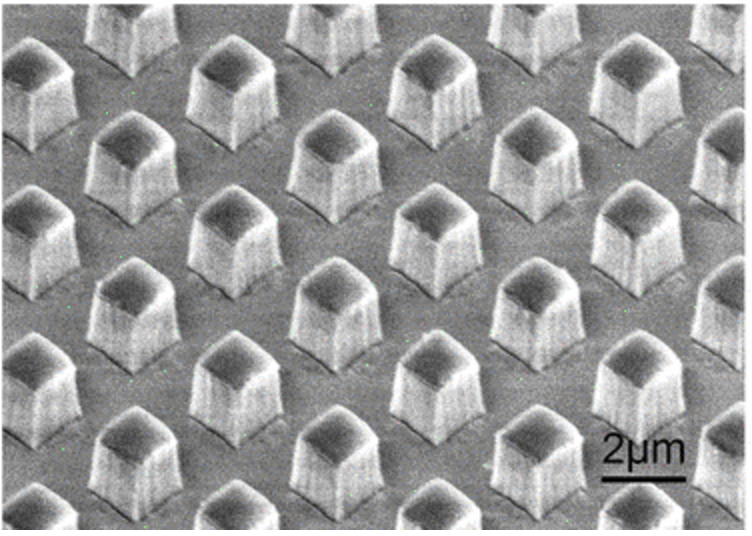
\includegraphics[width=.7\textwidth]{img/Ginn}
	\caption{Первая полностью диэлектрическая структура с оптическим магнетизмом \cite{Ginn2012}}
	\label{fig:ginn}
\end{figure}

Как уже упоминалось выше, впервые ненулевой магнитный дипольный момент в исключительно диэлектрическом метаматериале был экспериментально получен Джеймсом Джинном (англ. James C. Ginn) и соавторами и описан в статье \cite{Ginn2012}. Структурно среда представляла из себя массив теллуровых кубических резонаторов, показанный на рисунке \ref{fig:ginn}. Оптический магнетизм в видимом и инфракрасном диапазонах впервые наблюдался для кремниевых наносфер \cite{Evlyukhin2012a, Kuznetsov2012}. Так как в этой спектральной области показатель преломления кремния достаточно велик, то выводы теории Ми о возникновении магнитного резонанса \cite{Zhao2009} применимы.

Теоретическое и экспериментальное рассмотрение интерференции электрического и магнитного дипольных резонансов отдельных кремниевых нанодисков субволновых масштабов было осуществлено в работе \cite{Staude2013}. Наноструктуры были изготовлены по распространённой технологии ''кремния на изоляторе``. Была показана зависимость спектрального расположения резонансов в спектре коэффициента пропускания от диаметра нанодисков, а форма этих линейных спектров может быть объяснена через рассмотрение деструктивной интерференции двух резонансов. С помощью метода конечных интегралов в частотной области (FIFD) было рассчитано распределение электрической и магнитной компонент локального поля внутри кремниевого нанодиска.

В работе \cite{Habteyes2014} методом безапертурной ближнепольной оптической микроскопии было исследовано распределение амплитуды и фазы локализованных оптических мод в кремниевых нанодисках, аналогичных описанным и рассмотренным в статье \cite{Staude2013}. Исследование проводилось в диапазоне длин волн от 0.5 мкм до 1.0 мкм, также были получены оценки для вкладов магнитных и электрических диполей, квадруполей и октуполей: выявилось доминирование электрического квадрупольного резонанса, что подтверждалось численными расчётами, основанными на разложении рассеянного поля в ряд сферических функций.

В \cite{Evlyukhin2014} рассматривалось влияние поляризации взаимодействующего электромагнитного излучения и угла падения на рассеяние света кремниевыми наноцилиндрами субволновых размеров. Проведённый мультипольный анализ экспериментального спектра рассеяния, основанный на разложении по приближению дискретных диполей, подтвердил резонансное возбуждение электрических и магнитных мод в наноцилиндрах, также было показано что зависимость возбуждения резонансов от угла падения и поляризации позволяет управлять рассеянным светом в подобной системе.